\documentclass[a4paper, 11pt]{article}
%packages used
\usepackage[utf8]{inputenc}
\usepackage[T1]{fontenc}
\usepackage[top=2cm, bottom=2cm, left=2cm, right=2cm]{geometry}
\usepackage{graphicx}
\usepackage{amsmath, amssymb}
\usepackage{bm}
\usepackage[pdftex, bookmarks, colorlinks, breaklinks]{hyperref}
\usepackage{fancyhdr}
\usepackage{titlesec}
\usepackage{tocloft}
\usepackage{listings}
\usepackage{sudoku}
\usepackage{array}
\usepackage{indentfirst}
\usepackage{longtable}
\usepackage{multirow}
\usepackage{xcolor}
\usepackage{hyperref}

% Adjust section and subsection formatting

\titleformat{\section}[block]{\normalfont\Large\bfseries}{\hspace{1em}\thesection}{1em}{}
\titleformat{\subsection}[block]{\normalfont\large\bfseries}{\hspace{2em}\thesubsection}{1em}{}
\titlespacing*{\section}{0pt}{\baselineskip}{\baselineskip}
\titlespacing*{\subsection}{0pt}{\baselineskip}{\baselineskip}

%defining stuff
\pagecolor{white}
\newcolumntype{B}{>{\ttfamily\centering\arraybackslash}p{1em}}
\hypersetup{
    colorlinks = true,
    linkcolor = blue
}
\lstset{
    language=C,
    basicstyle=\ttfamily,
    morekeywords={size_t, colors_t, FILE},
    %keywordstyle=\color{blue},
    commentstyle=\color{green},
    stringstyle=\color{red},
    numbers=left,
    numberstyle=\tiny,
    frame=single,
    breaklines=true,
    %keywordstyle=[2]{\color{mypurple}},
    %morekeywords=[2]{size_t, colors_t, FILE}, 
    }

% Set paragraph indentation and spacing
\setlength{\parindent}{1em}
\setlength{\parskip}{1em}
\setlength\sudokusize{7cm}

% Page style configuration
\fancyhf{}
\pagestyle{fancy}
\rhead{\thepage}
\lhead{\leftmark}

\title{Master CSI}
\date{}  %empty string to make nothing appear

\begin{document}
\maketitle
\thispagestyle{empty}  % No page number on the title page

\begin{center}
    \hrule %thick line before
    \vspace{1\baselineskip}
    {\Huge\bfseries Sudoku Project Report}  % Title (changed from \Huge to \Large)
    
    \vspace{1\baselineskip}  % Adjust the vertical space after the line
    \hrule  % Thick line after the title
    \vspace{1\baselineskip}  % Adjust the vertical space after the line
    
    \vspace{2\baselineskip} 
    
\includegraphics[width=10cm]{university_logo.png}  % Set the width to your preference
 
    \vspace{6\baselineskip}  % Adjust the vertical space as needed
    
    \large
    A report submitted to the University of Bordeaux \\
    in partial fulfillment of the requirements for the course \\
    conducted by Prof. Emmanuel FLEURY \\
    
    \vspace{5\baselineskip}  % Adjust the vertical space after the line
    Written by Corentin CHAZAL \\
    
    \vspace{5\baselineskip}  % Adjust the vertical space after the line
    Department of Computer Science \\
    Faculty of Science and Technology \\
    University of Bordeaux \\
    
    \vspace{4\baselineskip}  % Adjust the vertical space after the line
    \date{November 24, 2023}
\end{center}

\newpage

\tableofcontents

\newpage

\vspace{3\baselineskip}
\section{Objectives}
The main objectives of the Sudoku Project are as follows:
\begin{itemize}
    \item Develop a Sudoku solver/generator.
    \item Ensure the solver can handle grids ranging from 1x1 to 64x64.
    \item Enable the solver to solve input grids.
    \item Implement a generator capable of creating Sudoku grids with a filling rate of 75, with a unique solution or multiple.
\end{itemize}

\begin{figure}[h]
  \centering
  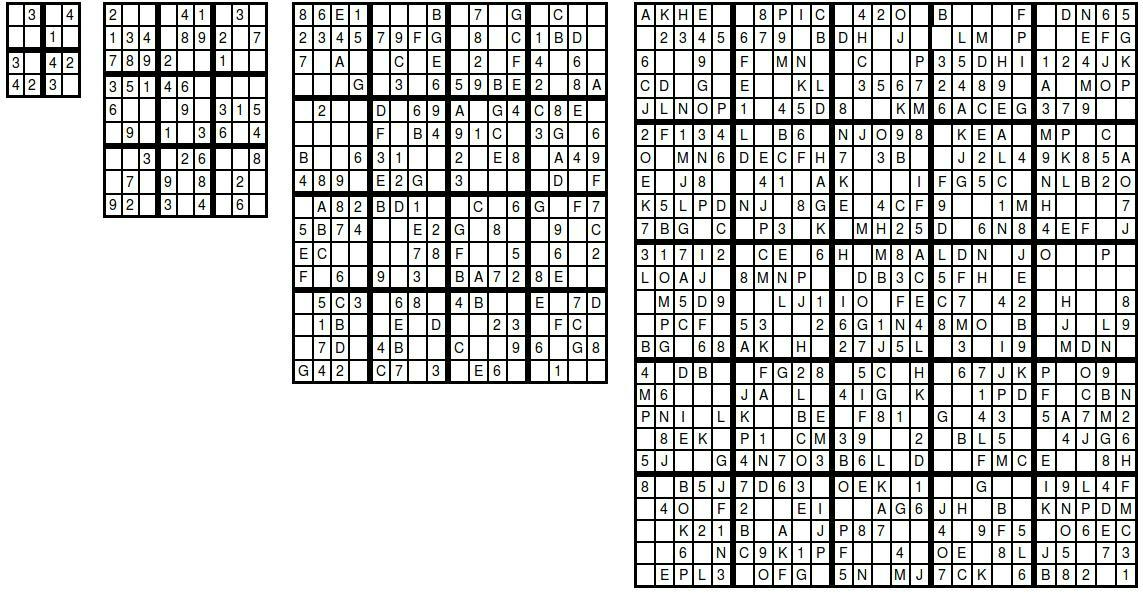
\includegraphics[width=0.8\textwidth]{grilles.png}
  \caption{Example of Sudoku grids to be solved.}
\end{figure}

\section{Approach}
In this section, we will discuss the approach taken to solve the Sudoku problem, including the use of bit hacks, heuristics, the parser, and the challenges faced.

\subsection{Parser}
A parser is implemented to handle the input of Sudoku grids. This component reads and interprets the given grids, allowing the solver to process and solve them.

In the grid parser, the idea is to get the first line of the file to determine the size, allocate a grid, and fill its first row accordingly. The parser then traverses the entire file to fill the rest of the grid with the determined size. This process involves managing various error and inconsistency cases, such as missing lines, invalid characters, and extra lines. The implementation strives for clean code, minimizing redundancy, and employs techniques like a \texttt{switch case}  on different characters to avoid code duplication. Despite the complexity, with 154 lines of code and several loops, there may be opportunities for further optimization.

\begin{figure}[h]
  \centering
  \begin{lstlisting}[language=C, frame = single, numbers = left, label=code:Example]
  static void cleaning(FILE *filename, grid_t *grid) {
    if (filename != NULL) {
      fclose(filename);
    }

    if (grid != NULL) {
      grid_free(grid);
    }
  }
  \end{lstlisting}
  \caption{Cleaning Function}
  \end{figure}
Used to free grids and close files at almost every error cases in the \texttt{file parser}.

\subsection{Bit Hacks}
Bitwise operations are utilized to optimize certain operations in the Sudoku solver, providing a more efficient implementation. Using \texttt{long long unsigned} bits, we can represents cells of grids up to a size of 64 and apply operations more efficiently on cells.
Each set bit is a choice possible for that cell. If all bits are set, every choice is possible. If it is a singleton, the cell is "solved".

\begin{figure}[h]
\[
\begin{bmatrix}
0 & 1 & 0 & 0 & 0 & 0 & 1 & 1 & 1
\end{bmatrix}
\]
 \caption{Example of the colors of a cell in a grid of size 9}
\end{figure}



\subsection{Heuristics}
Various heuristics play a crucial role in enhancing the efficiency of the Sudoku solver. Four main heuristics were employed during the development: \texttt{cross hatching}, \texttt{lone number}, \texttt{naked subset}, and \texttt{hidden subset}. Each heuristic contributes to the systematic solving process.

\subsubsection{Cross Hatching}
\texttt{cross hatching} is a fundamental heuristic used to narrow down possible values for each cell. It involves scanning each row and column, eliminating values that are already present in the corresponding row or column. This heuristic significantly reduces the search space and facilitates the solving process.

\subsubsection{Lone Number}
The \texttt{lone number} heuristic focuses on identifying cells where a number can only appear once in a particular row, column, or subgrid. By iteratively applying this heuristic, the solver can deduce and fill cells with certainty, progressing towards the solution.

\subsubsection{Hidden Subset and Naked Subset}
\texttt{hidden subset} and \texttt{naked subset} heuristics deal with identifying sets of numbers that can only appear in a particular group of cells (either row, column, or subgrid). While these heuristics are powerful, they can be computationally expensive, especially in the case of \texttt{hidden subset}. Initially, \texttt{hidden subset} was excluded from the solver's strategies due to its potential impact on efficiency. However, it was later revisited for specific grid configurations where its application could significantly expedite the solving process.

\subsection{Above and beyond...}
Here are some other heuristics that could be implemented to go even further.
\subsubsection{Pointing Pairs/Box-Line Reduction}
This technique is used to eliminate candidate numbers in a box. If a candidate number appears in a row or column of a box and nowhere else in that row or column, then that candidate number can be eliminated from the rest of the row or column in that box. It leverages the fact that if a certain number is confined to a specific row or column within a box, it cannot appear in the same row or column outside the box.

\subsubsection{X-Wing}
X-Wing is a more advanced strategy that looks for patterns in candidate placements. If there are two rows or columns where a candidate appears exactly twice in the same two columns or rows, and those two rows or columns align, then the candidate can be eliminated from other cells in the intersecting columns or rows. This method takes advantage of the elimination possibilities created by the alignment of candidate occurrences.

\subsubsection{Y-Wing}
Y-Wing is a sophisticated technique that involves creating a chain of cells with candidate numbers. The chain consists of three cells, each linked by the elimination of candidate numbers. As a result, this chain allows for the deduction and elimination of other candidates. Y-Wing requires a deeper understanding of candidate relationships and is considered an advanced solving strategy.



\subsection{Backtrack}
The \texttt{backtrack} function is a crucial component of the Sudoku solver, implementing a backtracking algorithm. It explores possible solutions by making tentative choices, applying heuristics, and recursively navigating through the grid. The function continuously checks for consistency and applies subgrid heuristics until a valid solution is found. When a solution is detected, it increments the solution count and, depending on the mode, either prints the solution or returns it. The function gracefully handles choices, verbose printing, and discarding unsuccessful paths, contributing to the overall solving process.



\subsection{Generator}
There are multiple ways to implement the generator. One approach is to fill diagonals first, and another is to fill the first row first, then the first block, followed by the first column, and so on. In this implementation, we use the second approach.

The algorithm starts by generating an empty grid of the desired size. Initially, all cells are filled with full colors, making the grid completely empty. The generator then 'randomly' selects colors to be set in the first row, discarding and repeating this process until the first row is complete. The same procedure is applied to fill the first block and column.

For grids with non-unique solutions, the algorithm iteratively completes the grid using \texttt{backtrack}. Subsequently, cells are removed until the filling rate reaches 75\%. In the case of a unique solution, the generator repeats the process until a unique solution is achieved. It's worth noting that reducing the filling rate makes generating a grid with a unique solution exponentially difficult due to the increased number of choices available.


\begin{figure}[h]
  \centering
  \begin{sudoku}
    |9 |1 |2 |3 |4 |5 |6 |7 |8|.
    |4 |3 |5 | | | | | | |.
    |6 |7 |8 | | | | | | |.
    |2 | | | | | | | ||.
    |5 | | | | | | | ||.
    |8 | | | | | | | ||.
    |7 | | | | | | | ||.
    |3 | | | | | | | ||.
    |1 | | | | | | | ||.
  \end{sudoku}
  \caption{Example of a 9x9 grid with the first row, block, and column filled}
\end{figure}

The overall complexity of the generator is dominated by the backtracking step. If the backtracking algorithm has exponential complexity, the function's overall complexity would be exponential as well. The rest of the operations contribute polynomial factors to the overall complexity.

\section{Difficulties}
\par This section discusses the difficulties encountered during the development of the Sudoku solver. The most challenging parts included the \texttt{file parser}, heuristics, \texttt{backtrack}, generator, and the optimization of the code.

\par It was observed that without using the \texttt{hidden subset} heuristic, the program could solve challenging grids within seconds, including some large grids like 64 by 64. However, when \texttt{hidden subset} was applied, it expanded the range of solvable grids but significantly slowed down the program. Striking a balance between efficiency and generality posed a notable challenge.

\par Additionally, during the last homework, I encountered some memory leaks in the \texttt{backtrack} function because I wasn't freeing all grids that needed to be freed. I extensively used \texttt{valgrind} to track and resolve these memory leaks. To enhance code performance, I utilized the \texttt{- time} option to compare the program's execution times during code modifications.

\par The major changes I implemented included optimizing cross-hatching and adjusting the application of heuristics. \texttt{cross hatching} and \texttt{lone number} heuristics are applied in a loop until they can no longer modify the grid due to their speed. Subsequently, \texttt{naked subset} and \texttt{hidden subset} heuristics are employed. The program goes through cross-hatching the most times according to the \texttt{gcov} extension results, with a decreasing frequency for \texttt{hidden subset}. Interestingly, the code is faster in solving level 3 puzzles without using \texttt{hidden subset}, but struggles to solve complex grids of size 64 within a reasonable time.

\par Throughout this project, I faced several difficulties, with the least number of failed tests being \(5\), then \(11\). Consequently, I didn't score as many points on my program. During my last undergraduate year at Northern Arizona University, I became accustomed to their coding style, which, admittedly, was quite confusing. For instance, they didn't allow declaring index variables in loops; they had to be global in the function. Consequently, I had to readapt to the University of Bordeaux coding style, which initially cost me points on the first homework assignments. However, I found that reducing the variable scope makes more sense and improves code maintainability.

\begin{figure}[h]
  \centering
  \begin{lstlisting}[language=C, frame = single, numbers = left]
bool subgrid_heuristics(colors_t *subgrid[], const size_t size) {
  if (subgrid == NULL) {
    return false;
  }
  bool changes = false;

  while (1) {
    if (cross_hatching_heuristic(subgrid, size)) {
      changes = true;
      continue;
    }
    if (lone_number_heuristic(subgrid, size)) {
      changes = true;
      continue;
    }
    break;
  }

  while (naked_subset_heuristic(subgrid, size)) {
    changes = true;
  }
  while (hidden_subset_heuristic(subgrid, size)) {
    changes = true;
  }
  return changes;
}
  \end{lstlisting}
  \caption{Function optimized to apply heuristics}
  \end{figure} 
  
Reducing the usage of \texttt{hidden subset} without deleting it was a real challenge as well as writing in an efficient way the first part calling the fastest heuristics. Trying to call \texttt{hidden subset} if and only if \texttt{naked subset} was changing the grid led to tons of other issues even though it seemed pretty interesting doing it that way. 

\newpage

\section{Code Improvements}
\par The optimization process involved factorizing code with helper functions, utilizing \texttt{switch cases}, and leveraging properties of bits to optimize \texttt{cross hatching}, as shown below. In terms of heuristics, a strategic approach was adopted. \texttt{cross hatching} was applied first until it couldn't modify the grid further, given its efficiency. Subsequently, the \texttt{lone number} heuristic was employed in a similar manner. Finally, the \texttt{hidden subset} heuristic was applied at the end due to its significant impact on program performance.

\begin{figure}[h]
\begin{lstlisting}[language=C,frame = single, numbers = left]
 bool cross_hatching_heuristic(colors_t *subgrid[], size_t size) {
  colors_t singleton = colors_empty();
  bool changed = false;

  for (size_t row = 0; row < size; row++) {
    if (colors_is_singleton(*subgrid[row])) {
      singleton = colors_or(singleton, *subgrid[row]);
    }
  }

  if (singleton != 0) {
    for (size_t index = 0; index < size; index++) {
      if (!colors_is_singleton(*subgrid[index]) &&
          colors_and(singleton, *subgrid[index]) != 0) {

        *subgrid[index] = colors_subtract(*subgrid[index], singleton);
        changed = true;
      }
    }
  }
  return changed;
}
\end{lstlisting}
\caption{Cross-Hatching after optimization}
\end{figure}

\par Initially, the complexity of Cross Hatching was \(O(n^2)\), but through leveraging properties of the bit hack functions developed for the solver, it was refined to \(O(n)\). This optimization substantially improved the efficiency of the solver, particularly when dealing with larger grid sizes.
 
\newpage

\section{Statistics}
\par These tests have been done on \texttt{jolicoeur} by \texttt{remote ssh} so the execution time may differ depending on the machine.  
\title{Running challenges without \texttt{hidden subset}:}

\begin{figure}[h]
    \centering
    \begin{longtable}{|c|c|c|c|c|c|}
        \hline
        \multirow{2}{*}{\textbf{Level}} & \multirow{2}{*}{\textbf{Test}} & \multicolumn{3}{c|}{\textbf{Results (s)}} & \multirow{2}{*}{\textbf{Average (s)}} \\
        \cline{3-5}
        & & \textbf{Real} & \textbf{User} & \textbf{System} & \\
        \hline
        \endfirsthead
        % Header on subsequent pages
        \hline
        \multirow{2}{*}{\textbf{Level}} & \multirow{2}{*}{\textbf{Test}} & \multicolumn{3}{c|}{\textbf{Results (s)}} & \multirow{2}{*}{\textbf{Average (s)}} \\
        \cline{3-5}
        & & \textbf{Real} & \textbf{User} & \textbf{System} & \\
        \hline
        \endhead
        % Footer on subsequent pages
        \hline
        \endfoot

        % Data for level 1 (without hidden subset)
        \multirow{3}{*}{1} & 1 & 0m1.334s & 0m0.013s & 0m0.019s & \multirow{3}{*}{\textbf{0.464}} \\
        \cline{2-5}
        & 2 & 0m0.035s & 0m0.020s & 0m0.008s & \\
        \cline{2-5}
        & 3 & 0m0.024s & 0m0.010s & 0m0.006s & \\
        \hline

        % Data for level 2 (without hidden subset)
        \multirow{3}{*}{2} & 1 & \textbf{Way too slow!} & & & \multirow{3}{*}{\textbf{Way too slow!}} \\
        \cline{2-5}
        & 2 & \textbf{Way too slow!} & & & \\
        \cline{2-5}
        & 3 & \textbf{Way too slow!} & & & \\
        \hline

        % Data for level 3 (without hidden subset)
        \multirow{3}{*}{3} & 1 & 1m14.030s & 1m4.215s & 0m6.967s & \multirow{3}{*}{\textbf{1m12.474}} \\
        \cline{2-5}
        & 2 & 1m11.558s & 1m0.717s & 0m7.234s & \\
        \cline{2-5}
        & 3 & 1m11.833s & 1m1.899s & 0m7.266s & \\
        \hline

        % Data for level 4-5 (without hidden subset)
        \multirow{3}{*}{4-5} & 1 & \textbf{Way too slow!} & & & \multirow{3}{*}{\textbf{Way too slow!}} \\
        \cline{2-5}
        & 2 & \textbf{Way too slow!} & & & \\
        \cline{2-5}
        & 3 & \textbf{Way too slow!} & & & \\
        \hline
    \end{longtable}
    \caption{Solving mode statistics without \texttt{hidden subset}}
\end{figure}

\title{Running challenges with \texttt{hidden subset}:}
\begin{figure}[h]
    \centering
    \begin{longtable}{|c|c|c|c|c|c|}
        \hline
        \multirow{2}{*}{\textbf{Level}} & \multirow{2}{*}{\textbf{Test}} & \multicolumn{3}{c|}{\textbf{Results (s)}} & \multirow{2}{*}{\textbf{Average (s)}} \\
        \cline{3-5}
        & & \textbf{Real} & \textbf{User} & \textbf{System} & \\
        \hline
        \endfirsthead
        % Header on subsequent pages
        \hline
        \multirow{2}{*}{\textbf{Level}} & \multirow{2}{*}{\textbf{Test}} & \multicolumn{3}{c|}{\textbf{Results (s)}} & \multirow{2}{*}{\textbf{Average (s)}} \\
        \cline{3-5}
        & & \textbf{Real} & \textbf{User} & \textbf{System} & \\
        \hline
        \endhead
        % Footer on subsequent pages
        \hline
        \endfoot

        % Data for level 1 (with hidden subset)
        \multirow{3}{*}{1} & 1 & 0m0.040s & 0m0.005s & 0m0.023s & \multirow{3}{*}{\textbf{0.036}} \\
        \cline{2-5}
        & 2 & 0m0.035s & 0m0.017s & 0m0.011s & \\
        \cline{2-5}
        & 3 & 0m0.033s & 0m0.010s & 0m0.017s & \\
        \hline

        % Data for level 2 (with hidden subset)
        \multirow{3}{*}{2} & 1 & \textbf{Way too slow!} & & & \multirow{3}{*}{\textbf{Way too slow!}} \\
        \cline{2-5}
        & 2 & \textbf{Way too slow!} & & & \\
        \cline{2-5}
        & 3 & \textbf{Way too slow!} & & & \\
        \hline

        % Data for level 3 (with hidden subset)
        \multirow{3}{*}{3} & 1 & 1m15.854s & 1m7.974s & 0m7.090s & \multirow{3}{*}{\textbf{1m15.522}} \\
        \cline{2-5}
        & 2 & 1m17.169s & 1m9.013s & 0m7.270s & \\
        \cline{2-5}
        & 3 & 1m13.543s & 1m5.272s & 0m6.760s & \\
        \hline

        % Data for level 4-5 (with hidden subset)
        \multirow{3}{*}{4-5} & 1 & \textbf{Way too slow!} & & & \multirow{3}{*}{\textbf{Way too slow!}} \\
        \cline{2-5}
        & 2 & \textbf{Way too slow!} & & & \\
        \cline{2-5}
        & 3 & \textbf{Way too slow!} & & & \\
        \hline
    \end{longtable}
    \caption{Solving mode statistics with \texttt{hidden subset}}
\end{figure}


\title{Grid generation of size 36 by 36:}

\begin{figure}[h]
    \centering
    \begin{longtable}{|c|c|c|c|}
        \hline
        \textbf{Grid} & \textbf{Real} & \textbf{User} & \textbf{System} \\
        \hline
        \endfirsthead
        % Header on subsequent pages
        \hline
        \textbf{Grid} & \textbf{Real} & \textbf{User} & \textbf{System} \\
        \hline
        \endhead
        % Footer on subsequent pages
        \hline
        \endfoot

        % Data for grids with multiple solutions
        1 & 0m3.171s & 0m3.109s & 0m0.038s \\
        2 & 0m2.886s & 0m2.819s & 0m0.035s \\
        3 & 0m2.791s & 0m2.749s & 0m0.039s \\
        \hline
    \end{longtable}
    \caption{Grid Generation Statistics (Multiple Solutions) with 75\% filling rate}
\end{figure}

\begin{figure}[h]
    \centering
    \begin{longtable}{|c|c|c|c|}
        \hline
        \textbf{ Grid } & \textbf{ Real } & \textbf{ User } & \textbf{ System } \\
        \hline
        \endfirsthead
        % Header on subsequent pages
        \hline
        \textbf{Grid} & \textbf{Real} & \textbf{User} & \textbf{System} \\
        \hline
        \endhead
        % Footer on subsequent pages
        \hline
        \endfoot

        % Data for grids with a unique solution
        1 & 0m2.930s & 0m2.904s & 0m0.024s \\
        2 & 0m15.387s & 0m15.304s & 0m0.047s \\
        3 & 0m2.678s & 0m2.647s & 0m0.030s \\
        \hline
    \end{longtable}
    \caption{Grid Generation Statistics (Unique Solution) with 75\% filling rate}
\end{figure}

\end{document}
